\documentclass[titlepage]{tufte-book}

\usepackage[runall=true]{pythontex}
\setpythontexworkingdir{<outputdir>}
\usepackage{environ}
\usepackage{morewrites}
\usepackage{amsthm}
\usepackage{amsmath}
\usepackage{amssymb}
\usepackage[pdftex]{graphicx}
\usepackage{epstopdf}
\usepackage{hyperref}
\usepackage{alltt}
\usepackage{listings}
\usepackage{array}
\usepackage{extarrows}
\usepackage{setspace}
\usepackage{tikz}
\usepackage{tikz-qtree}
\usetikzlibrary{calc}
\usetikzlibrary{positioning}
\usepackage{hyperref}
\usepackage{graphviz}
\usepackage{geometry}                % See geometry.pdf to learn the layout options. There are lots.
\usepackage{bashful}
\usepackage{microtype} % Improves character and word spacing
\usepackage{caption}

\usepackage{booktabs} % Better horizontal rules in tables

\setkeys{Gin}{width=\linewidth,totalheight=\textheight,keepaspectratio} % Improves figure scaling
\graphicspath{{images/}}

\usepackage{fancyvrb} % Allows customization of verbatim environments
\fvset{fontsize=\normalsize} % The font size of all verbatim text can be changed here

\newcounter{problem}
\newcounter{total}
\newcommand{\step}[1]{{}
\vspace{4pt} \noindent {\bf \theproblem. }#1\addtocounter{problem}{1}}

\newcommand{\cut}[1]{}

\usepackage[tikz]{bclogo}
\usepackage{tikz}
\usetikzlibrary{calc}

\lstdefinestyle{BashInputStyle}{
  language=bash,
  basicstyle=\small\ttfamily,
  numberstyle=\tiny,
  showstringspaces=false,
  numbersep=3pt,
  otherkeywords={|, ;, ', ", *,>, <, *, &, `, $},
  alsoletter={:~_},
  columns=fullflexible,
  backgroundcolor=\color{yellow!20},
  linewidth=0.93\linewidth,
  xleftmargin=0.03\linewidth,
  keywordstyle=\color{blue},
  emph={ls, cat, head, tail, more, less, sort, uniq, kill java, grep, zip, unzip, tar, wc, cp, chmod,chown},
  emphstyle=\color{black}\bfseries,
    commentstyle=\color{gray}\slshape
    }

\newcommand{\chili}{\scalebox{.04}{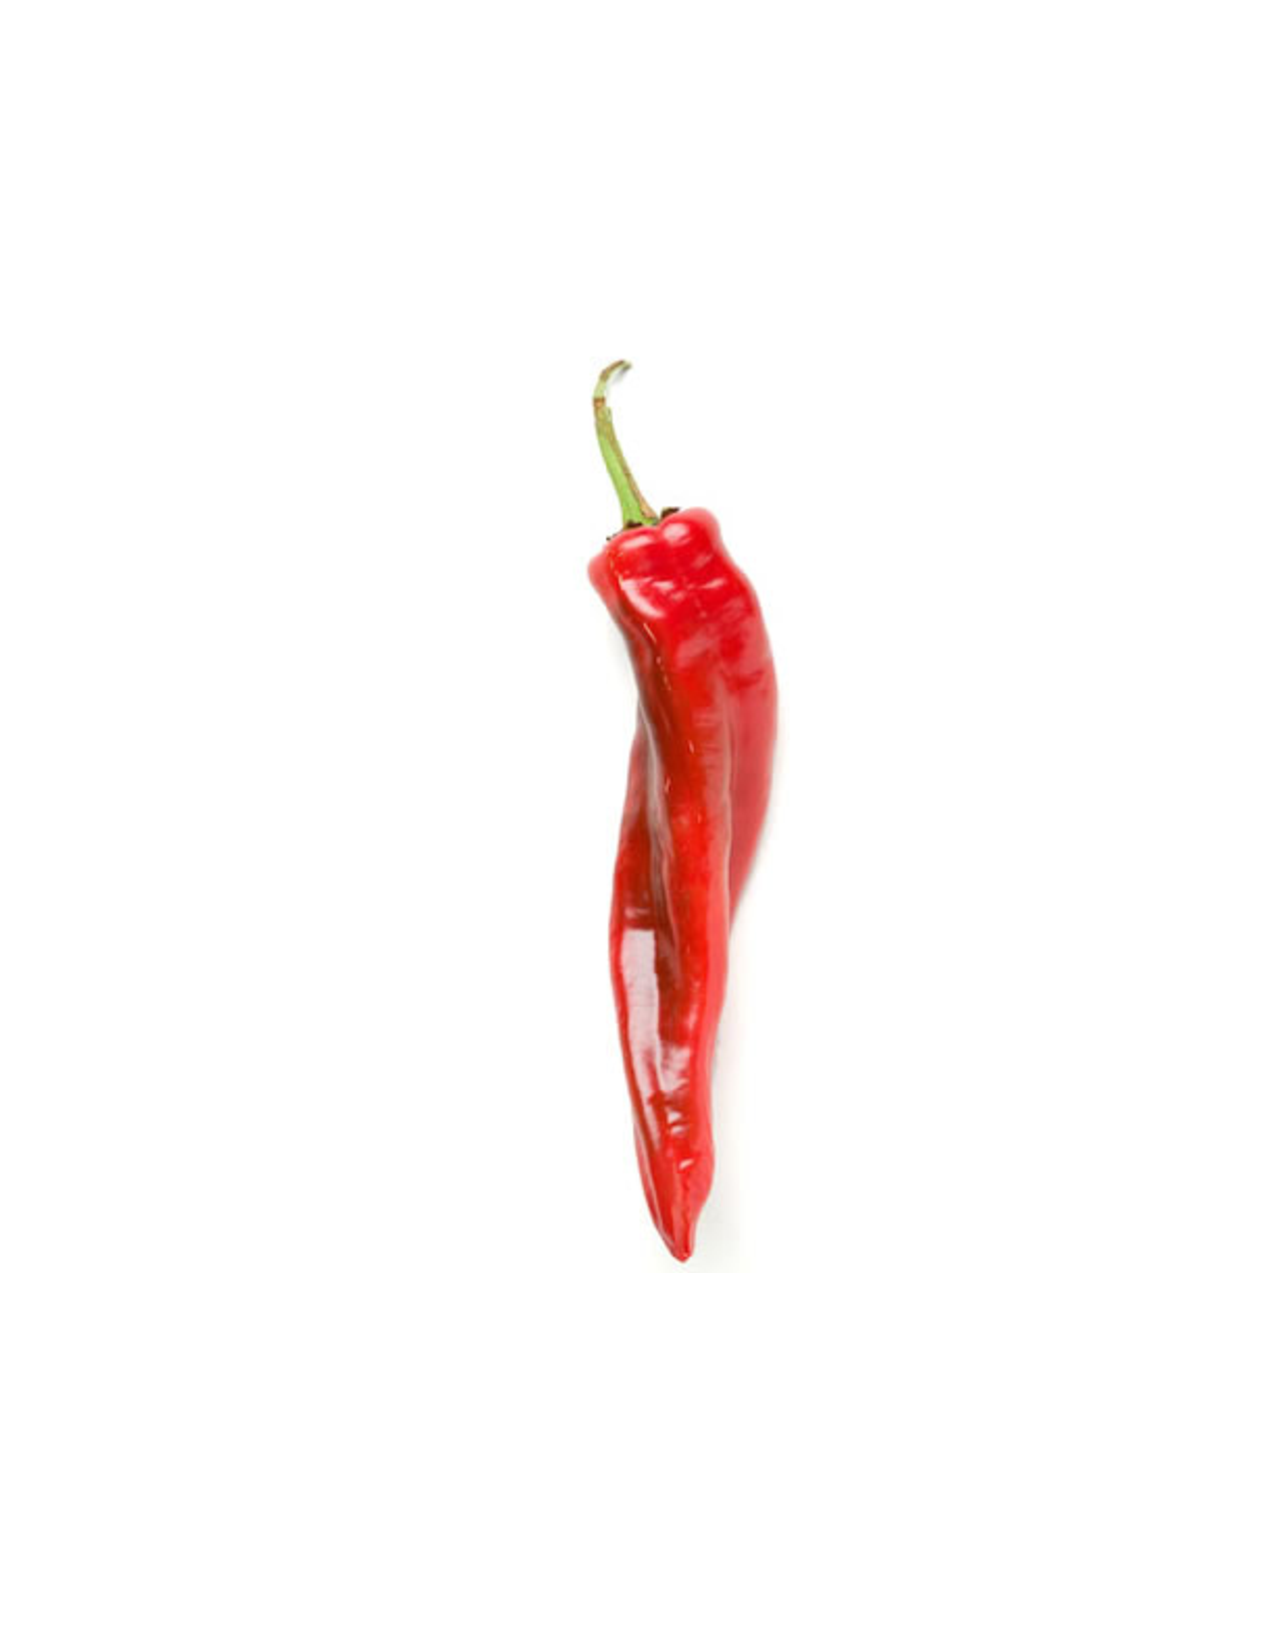
\includegraphics{images/chili.pdf}}}
\newcommand{\chchili}{{\chili\chili}}
\newcommand{\chchchili}{{\chchili\chili}}

% The units package provides nice, non-stacked fractions and better spacing
% for units.
\usepackage{units}

% The fancyvrb package lets us customize the formatting of verbatim
% environments.  We use a slightly smaller font.
\usepackage{fancyvrb}
\fvset{fontsize=\normalsize}

% Small sections of multiple columns
\usepackage{multicol}

\hypersetup{
urlcolor=blue,
colorlinks=true
}
\usepackage[noline, procnumbered, linesnumberedhidden, boxed]{algorithm2e}

\newcommand{\openepigraph}[2]{ % This block sets up a command for printing an epigraph with 2 arguments - the quote and the author
\begin{fullwidth}
\sffamily\large
\begin{doublespace}
\noindent\allcaps{#1}\\ % The quote
\noindent\allcaps{#2} % The author
\end{doublespace}
\end{fullwidth}
}

\newcommand{\figref}[1]{Figure~\ref{#1}}
\renewcommand{\thefigure}{\arabic{figure}}

\newenvironment{callout}[1]{
\[
  \left[
      \begin{tabular}{@{\quad}m{.05\textwidth}@{\qquad}m{.75\textwidth}@{\quad}}
        \scalebox{1.5}{#1} & 
          \raggedright%
}
{
      \end{tabular}
    \right]
\]
}

\newcommand{\blankpage}{\newpage\hbox{}\thispagestyle{empty}\newpage} % Command to insert a blank page

\usepackage{makeidx} % Used to generate the index
\makeindex % Generate the index which is printed at the end of the document

\renewcommand{\maketitlepage}[0]{%
  \cleardoublepage%
  {%
  \sffamily%
  \begin{fullwidth}%
  ~
  \vspace{11.5pc}%
  \fontsize{36}{40}\selectfont\par\noindent\textcolor{darkgray}{\allcaps{\thanklesstitle}}%
  
\scalebox{.2}{\includegraphics{images/msan-logo}}
  \vspace{11.5pc}%
  \fontsize{12}{18}\selectfont\par\indent\textcolor{darkgray}{\allcaps{\thanklessauthor}\\
\indent{\tt parrt@cs.usfca.edu}\\
\href{http://parrt.cs.usfca.edu}{http://parrt.cs.usfca.edu}}%
  \vspace{11.5pc}%
  \fontsize{14}{16}\selectfont\par\noindent\allcaps{\thanklesspublisher}%
  \end{fullwidth}%
  }
  \thispagestyle{empty}%
  \clearpage%
}

\titlecontents{part}% FIXME
    [0em] % distance from left margin
    {\vspace{1.5\baselineskip}\begin{fullwidth}\LARGE\rmfamily\itshape} % above (global formatting of entry)
    {\contentslabel{2em}} % before w/label (label = ``II'')
    {} % before w/o label
    {\rmfamily\upshape\qquad\thecontentspage} % filler + page (leaders and page num)
    [\end{fullwidth}] % after

  \titlecontents{chapter}%
    [0em] % distance from left margin
    {\vspace{1.5\baselineskip}\begin{fullwidth}\Large\rmfamily\itshape} % above (global formatting of entry)
    {\hspace*{0em}\contentslabel{2em}} % before w/label (label = ``2'')
    {\hspace*{4em}} % before w/o label
    {\rmfamily\upshape\qquad\thecontentspage} % filler + page (leaders and page num)
    [\end{fullwidth}] % after

\titlespacing*{\chapter}{0pt}{0pt}{30pt}
\titlespacing*{\section}{0pt}{3.5ex plus 1ex minus .2ex}{2.3ex plus .2ex}
\titlespacing*{\subsection}{0pt}{3.25ex plus 1ex minus .2ex}{1.5ex plus.2ex}

\begin{document}

\chapter{Iterative Optimization Via Gradient Descent}

\begin{fullwidth}

The goal of this lecture/lab is to solve an iterative computation problem with nontrivial iteration and termination conditions: {\em gradient descent function minimization}. 

\section{Discussion}

Finding $x$ that minimizes or "optimizes" function $f(x)$ (usually over some range) is an incredibly important operation as we use it to minimize risk and, for machine learning, to learn the parameters of our classifiers or predictors. For example, deep learning uses cost function optimization to train neural networks. Generally $x$ will be a vector but we will assume $x$ is a scalar to learn the basics. If we know that the function is convex like a quadratic polynomial, there is a unique solution and we can simply set the derivative equal to zero and solve for $x$:

\[\tag{Analytic solution to optimization}
f'(x) = 0
\]

\noindent That is basically asking the question, ``Where does the function flatten out?''  For example, the function $f(x) = (x-2)^2 + 1$ has derivative $f'(x) = 2x - 4$ whose zero is $x=2$.

\begin{center}
\scalebox{.25}{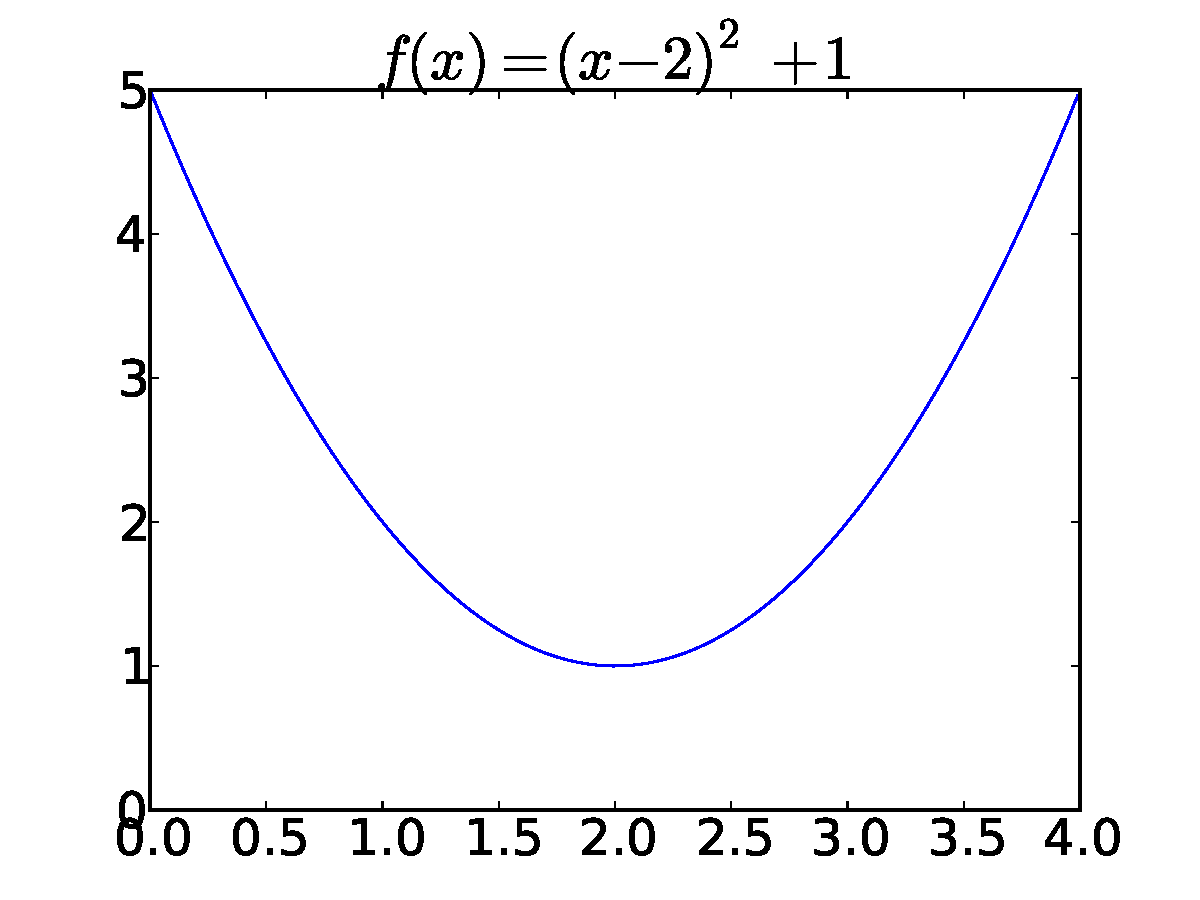
\includegraphics{images/quadratic.pdf}}
\end{center}

We prefer to find the {\em global minimum} but generally have to be satisfied with a {\em local minimum}, which we hope is close to the global minimum. A decent approach to finding the global minimum is to find a number of local minima via random starting $x_0$ locations and just choose the minimum local of the minima discovered. For example, the function $f(x) = cos(3\pi x) / x$ has two minima in $[0,1.1]$, with one obvious global minimum:

\begin{center}
\scalebox{.29}{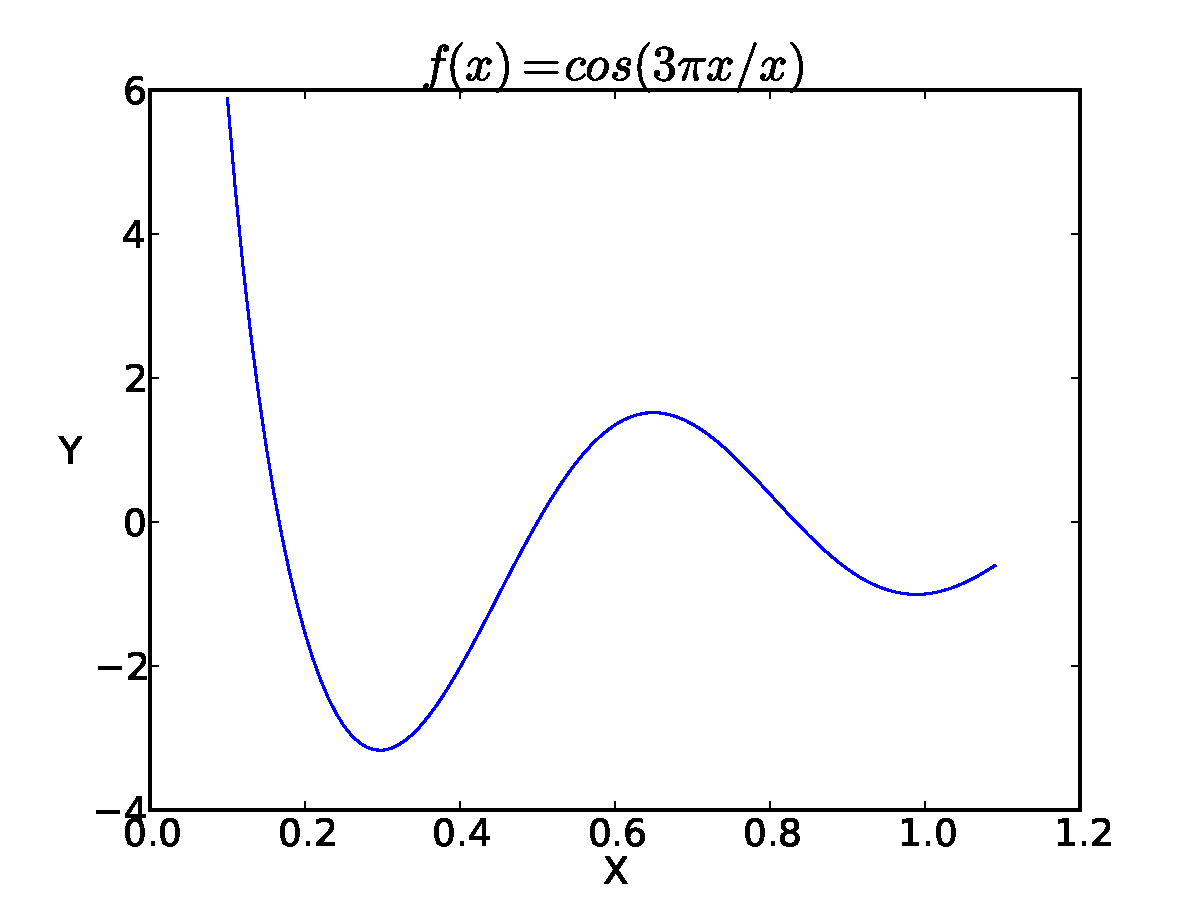
\includegraphics{images/cos-2minima.pdf}}
\scalebox{.29}{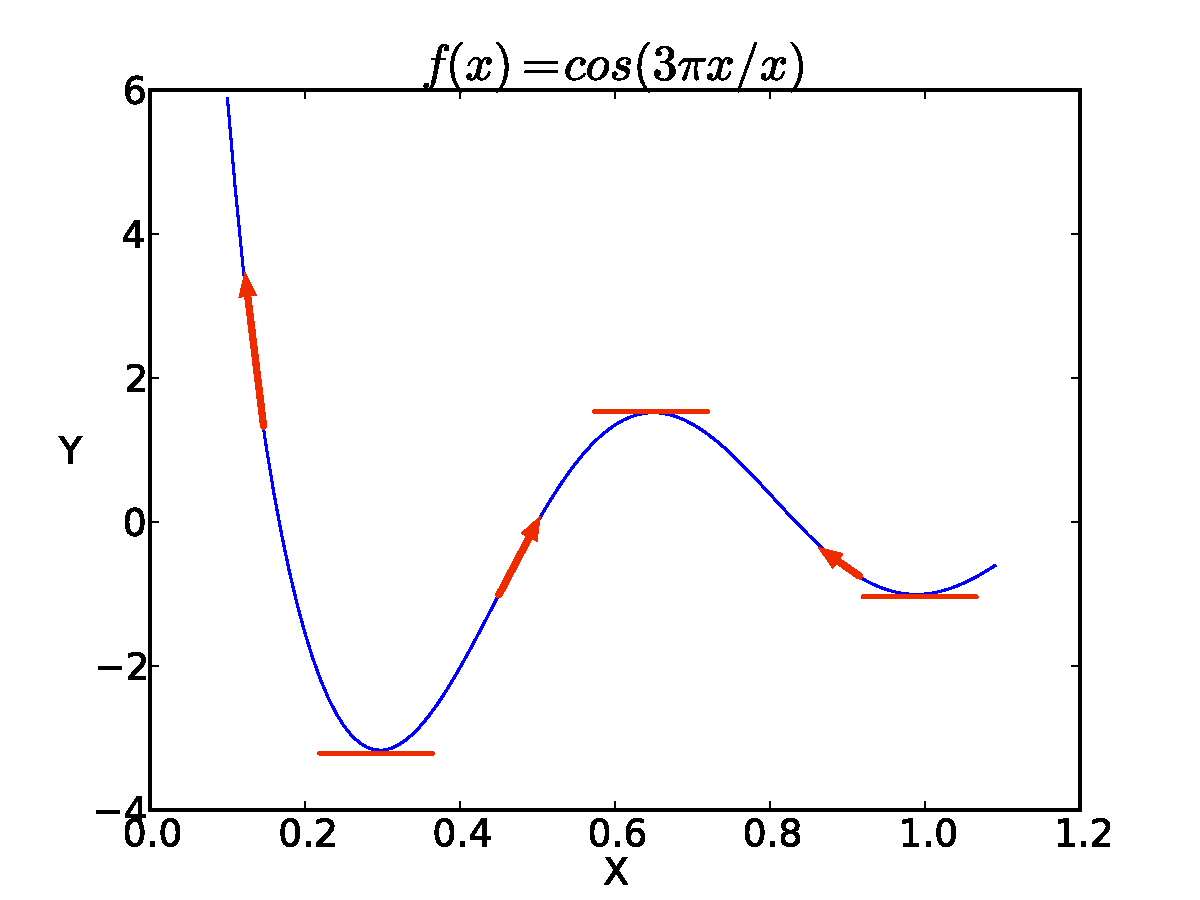
\includegraphics{images/cos-2minima-edited.pdf}}
\end{center}

If the function has lots of minima/maxima or is very complicated, there may be no easy analytic solution.
There are many approaches to finding function minima iteratively (i.e., non-analytically), but we will use a well-known technique called {\em gradient descent} or {\em method of steepest descent}.  

\subsection{Gradient descent}

This technique can be used to train everything from {\em linear regression} models (see one of your projects) to {\em neural networks}.  Gradient descent requires a starting position, $x_0$, the function to optimize, $f(x)$, and its derivative $f'(x)$.  Recall that the derivative is just the slope of a function at a particular point. In other words, as $x$ shifts away from a specific position, does $y$ go up or down, and by how much?  E.g., the derivative of $x^2$ is $2x$, which gives us a positive slope when $x>0$ and a negative slope when $x<0$.  Gradient descent uses the derivative to iteratively pick a new value of $x$ that gets us closer and closer to the minimum of $f(x)$.   The negative of the slope (in $y$) tells us the direction (in $x$) of the nearest minimum. For example, the graph to the right above shows a number of vectors representing derivatives at particular points. Note that the derivative is zero, i.e. flat, at the minima (same is true for maxima). The recurrence relation for updating our estimate of $x$ that minimizes $f(x)$ is then just:

\[
x_{i+1} = x_i - \eta f'(x_i)
\]

\noindent where $\eta$ is called the {\em learning rate}, which we'll discuss below. The $\eta f'(x_{i})$ term represents the size of the step we take towards the minimum. 
The basic algorithm is:

\begin{enumerate}
\item Pick an initial $x_0$, let $x = x_0$
\item Let $x_{i+1} = x_i - \eta f'(x_i)$ until $f'(x_i)=0$
\end{enumerate}

That algorithm is extremely simple but knowing when to stop the algorithm is problematic when dealing with the finite precision of computers. Specifically, no two floating-point numbers are ever equal really. So $f'(x) = 0$ is always false. Usually we do something like $abs(x_{i+1} - x_i) < precision$ or when $abs(f(x_{i+1}) - f(x_i)) < precision$ where precision is some very small number like 0.0000001.  Personally, I like the concept of stopping when there is a very small vertical change {\bf and} $f(x_{i+1})$ is heading back up.

The steps we take are scaled by the learning rate $\eta$.  Yaser S. Abu-Mostafa has some \href{http://www.amlbook.com/slides/iTunesU_Lecture09_May_01.pdf}{great slides} and videos that you should check out. Here is his description on slide 21 of how the learning rate can affect convergence:

\scalebox{.60}{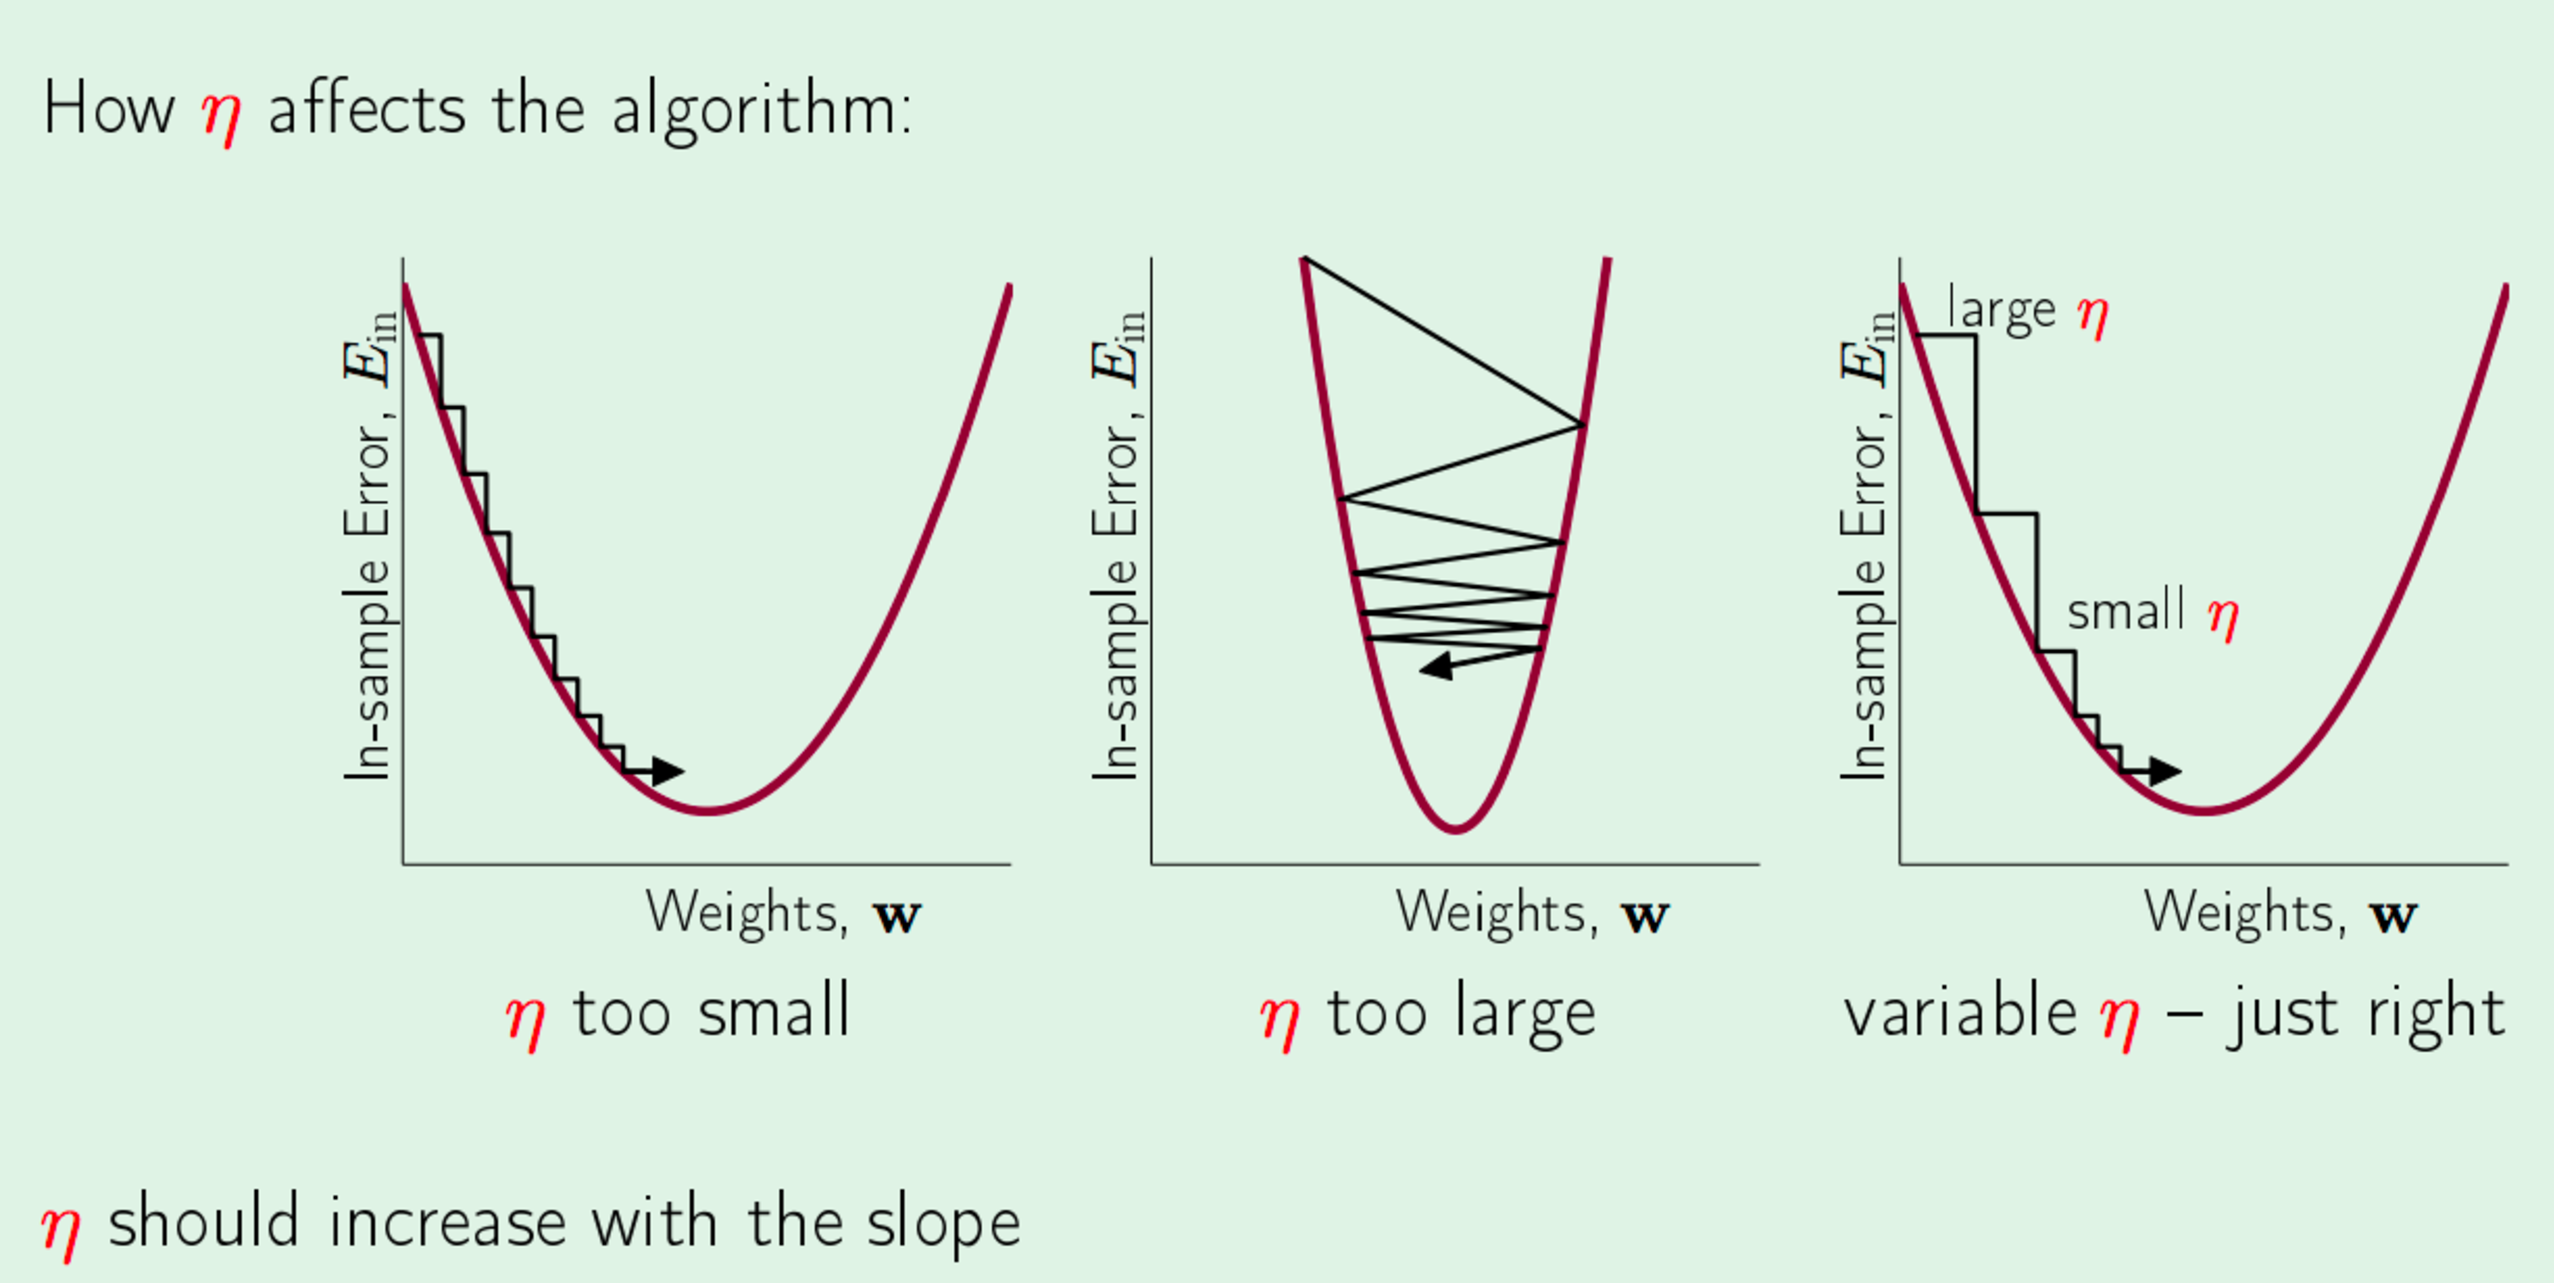
\includegraphics{images/stepsize.pdf}}

The domain of $x$ also affects the learning rate magnitude. This is all a very complicated finicky business and those experienced in the field tell me it's very much an art picking the learning rate, starting positions, precision, and so on. You can start out with a low learning rate and crank it up to see if you still converge without oscillating around the minimum.  \noindent An excellent description of gradient descent and other minimization techniques can be found in \href{http://apps.nrbook.com/fortran/index.html}{Numerical Recipes}.

\subsection{Approximating derivatives with finite differences}

Sometimes, the derivative is hard, expensive, or impossible to find analytically (symbolically).  For example, some functions are themselves iterative in nature or even simulations that must be optimized. There might be no closed form for $f(x)$. To get around this and to reduce the input requirements, we can approximate the derivative in the neighborhood of a particular $x$ value. That way we can optimize any reasonably well behaved function (left and right continuity would be nice). Our minimizer then only requires a starting location and $f(x)$ but not $f'(x)$, which makes the lives of our users much simpler and our minimizer much more flexible. 

To approximate the derivative, we can take several approaches. The simplest involves a comparison. Since we really just need a direction, all we have to do is compare the current $f(x_i)$ with values a small step, $h$, away in either direction: $f(x_{i}-h)$ and $f(x_{i}+h)$.  If $f(x_{i}-h) < f(x_{i})$, we should move $x_{i+1}$ to the left of $x_{i}$. If $f(x_{i}+h) < f(x_{i})$, we should move $x_{i+1}$ to the right.  This is called the forward difference but there is also backward difference and a central difference. The excellent article \href{http://research.microsoft.com/pubs/192769/tricks-2012.pdf}{\textcolor{blue}{Stochastic Gradient Descent Tricks}} has a lot of practical information on computing gradients etc...

Using the direction of the slope works, but does not converge very fast. What we really want is to use the magnitude of the slope to make the algorithm go fast where it's steep and slow where it's shallow because it will be approaching a minima. So, rather than just using the sign of the finite difference, we should use the magnitude or rate of change. Using finite differences then, we get a similar formula but replace the derivative with the finite (forward) difference:

\[
x _{i+1} = x_i - \eta \frac{f(x_{i}+h) - f(x_{i})}{h} \text{ where } f'(x) \approx \frac{f(x_{i}+h) - f(x_{i})}{h}
\]

\noindent To simplify things, we can roll the step size $h$ into the learning rate $\eta$ constant as we are going to pick that anyway.

\[
x _{i+1} = x_i - \eta (f(x_{i}+h) - f(x_{i}))
\]

\noindent  The step size is bigger when the slope is bigger and is smaller as we approach the minimum (since the region is flatter). Abu-Mostafa indicates in his slides that $\eta$ should increase with the slope whereas we are keeping it fixed and allowing the finite difference to increase the step size. We are not normalizing the derivative/difference to a unit vector like he does (see his slides).

\section{An implementation}

Our goal is to use gradient descent to minimize $f(x) = cos(3\pi x) / x$. To increase chances of finding the global minimum, we'll pick {\bf two} random locations in the range $[0.1,1.2]$ using standard python {\tt random.random()} and perform gradient descent with both of them. To  observe our minimizer in action, we'll plot of $f(x)$ with traces that indicate the steps taken by gradient descent. Here are two sample descents where the $x$ and $f(x)$ values are displayed as well as the minimum of those two:

\noindent \scalebox{.32}{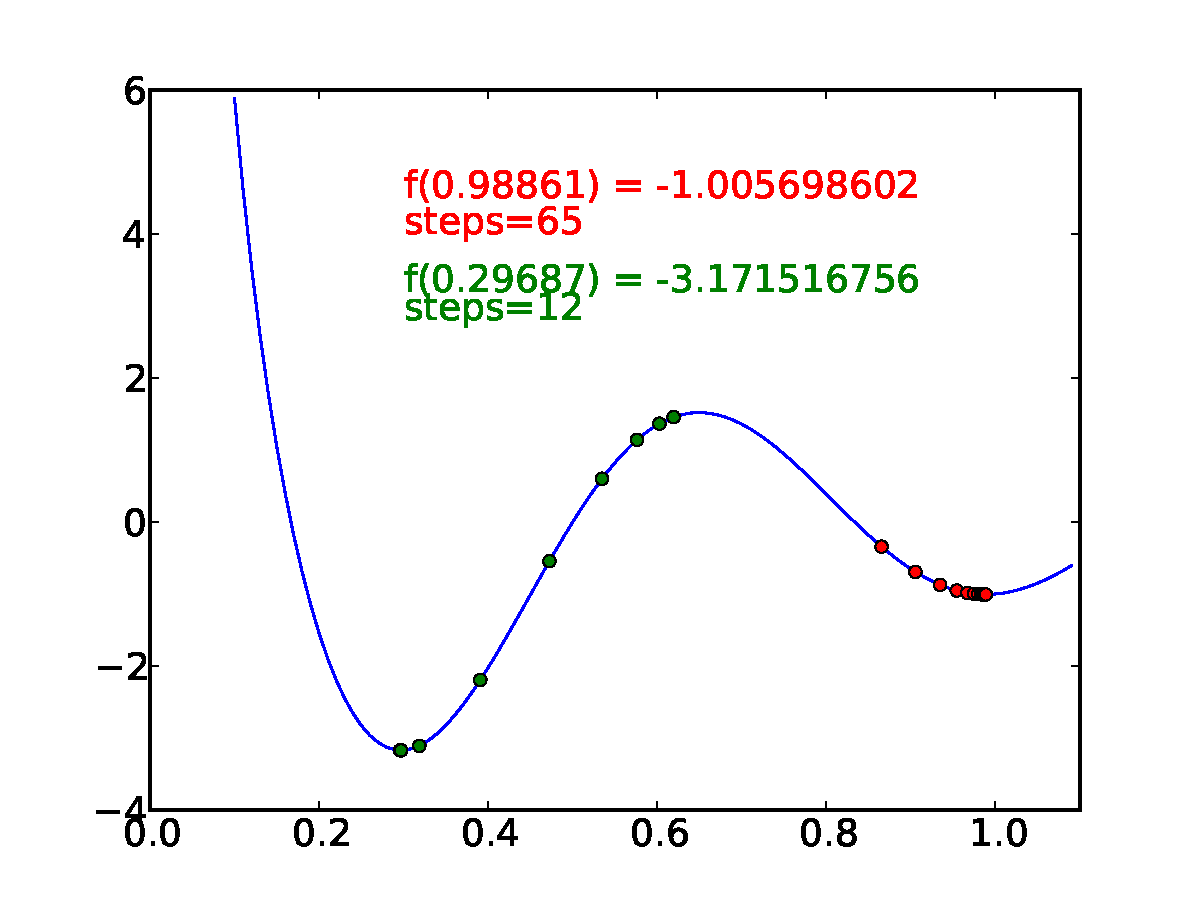
\includegraphics{images/cos-trace-2minima.pdf}}
\scalebox{.32}{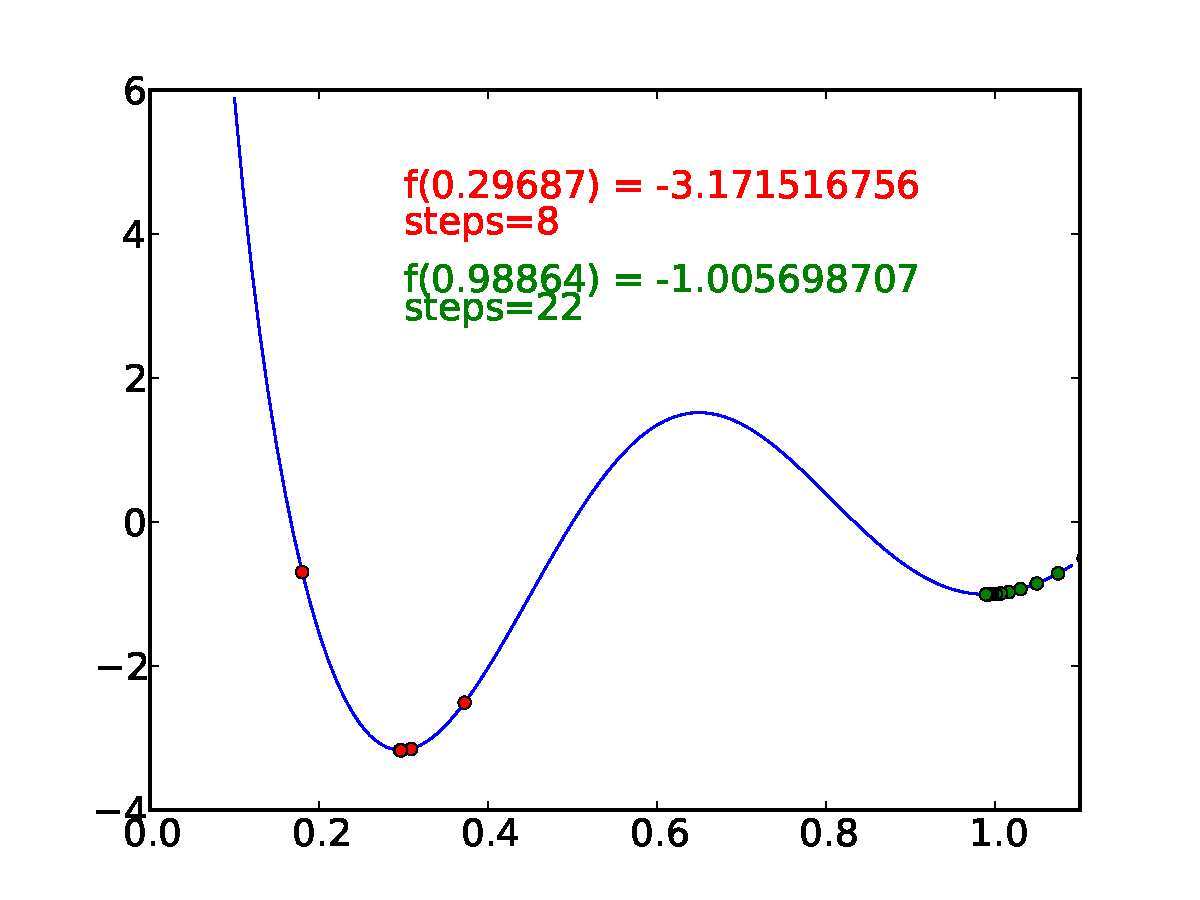
\includegraphics{images/cos-trace-2minima-left.pdf}}

\noindent Let's define a function called {\tt minimize} that takes the indicated parameters:

\begin{pyverbatim}
def minimize(f, x0, eta, h, precision):
    x = x0
    while True:
        prev = x
        finite_diff = f(x + h) - f(x)	 # division by h rolls into learning rate
        x = x - eta * finite_diff 		# decelerates x step as it flattens out
        delta = f(x) - f(prev)
        # stop when small change in vertical but not heading down
        if delta >= 0 and abs(delta) < precision: break
\end{pyverbatim}

\noindent Here's how we would call the minimize function:

\begin{pyverbatim}
ETA = 10
h = 0.0001
PRECISION = 0.0000001 # can't be too small as f(x)-f(xprev) prec is low
def f(x): return np.cos(3*np.pi*x) / x
x0 = runif(.1,1.2)  # using our uniform random number generator
minimize(f, x0, ETA, h, PRECISION)
\end{pyverbatim}

\noindent Notice how I snuck in that {\tt f()} definition for the above cosine function. I could have used a {\tt lambda} too:

\begin{pyverbatim}
minimize(lambda x : np.cos(3*np.pi*x) / x, x0, ETA, h, PRECISION)
\end{pyverbatim}

To visualize the cosine function, we can use the following.

\begin{pyverbatim}
import matplotlib.pyplot as plt

graphx = np.arange(.1,1.1,0.01)
graphy = f(graphx)
plt.plot(graphx,graphy)
plt.axis([0,1.1,-4,6])
\end{pyverbatim}

To create the ``trace'' dots we can just add the $x$ values to an array as we search for the minimum in {\tt minimize()} and return it to the caller:

\begin{pyverbatim}
def minimize(f, x0, eta, h, precision):
    tracex = []
    tracex.append(x0)
    ...
    while True:
        ...
        tracex.append(x)
        ...
\end{pyverbatim}

Then, we plot the trace ($x$, $f(x)$) pairs with red or green dots:

\begin{pyverbatim}
tracex = minimize(f, x0, ETA, h, PRECISION)
tracey = [f(x) for x in tracex]
plt.plot(tracex, tracey, 'ro') # plot red dots
\end{pyverbatim}

Choosing an appropriate step value $h$ is important to get a decent approximation of the derivative through finite differences but that is large enough to avoid faulty results from lack of precision (subtracting two floating-point numbers in the computer results in a number with much less precision than the original numbers). You want that number to be small enough so that your algorithm does not oscillate around the minimum. If the number is too big it will compute a finite difference that makes $x_{i+1}$ leap across the minimum to the other wall of the function.  We must also pick a learning rate $\eta$ that allows you to go as fast as we can but not so fast that it overruns the minimum back and forth. When I crank up my learning rate too far, I also see the algorithm oscillate:

\begin{pyverbatim}
...
f(0.491296576641) = -0.166774773584 , delta = 2.05763033375622805821
f(0.296744439739) = -3.171512867583 , delta = -3.00473809399913660556
f(0.297092626880) = -3.171512816769 , delta = 0.00000005081414267138
...
\end{pyverbatim}

To help you understand what your program is doing, print out $x$, $f(x)$, and any other value you think is helpful to see how your program explores the curve.umber

Your minimization function should converge in less than about 70 steps.

If you get really stuck piecing it together from the above, you can look at the [solution](https://github.com/parrt/msan501/blob/master/notes/code/descent.py).

\section{Testing}

There is some \href{https://github.com/parrt/msan501/blob/master/notes/code/test\_descent.py}{\textcolor{blue}{testing code}} available, which you run with {\tt pytest} module (that you might have to install):

\begin{verbatim}
$ python -m pytest test_descent.py 
======================================= test session starts =======================================
platform darwin -- Python 2.7.11 -- py-1.4.30 -- pytest-2.7.2
rootdir: /Users/parrt/github/msan501/notes/code, inifile: 
collected 12 items 

test_descent.py ............

==================================== 12 passed in 1.25 seconds ====================================
\end{verbatim}
 
\end{fullwidth}
\end{document}

